\section{Efficiency}

The goal of PIX is to provide a toolkit that enables the construction of
instrumentation tools that produce an efficient instrumented
executable. More importantly, one of the design goals of PIX is to genearte efficient instrumented executables
when number of instrumentation points is rather high  In this section, we describe the mechanism used in PIX 
to produce efficient instrumented executables.

\label{Subsection:Relocation}
\subsection{Code Relocation at Function Level}
The use of relocation at the function level in PIX stems from the fact
that we are performing the instrumentation statically on a platform that uses a
variable-length instruction set and it may not be always possible to instrument
an arbitrary point in the executable due to the lack of enough space for jump instruction to the instrumentation code. 
A typical strategy used by static
instrumentation tools on platforms with fixed-length instruction sets is to
replace a single fixed-length instruction at the instrumentation point with a
branch instruction that will transfer control to the instrumentation code. This is fairly straightforward because by the
definition of a fixed-length instruction set, the instruction being replaced and
the replacing jump have the same length. 
%Performing static instrumentation in a variable-length instruction set does not afford us this luxury. 
In x86 platforms, a
jump instruction that uses a 32-bit offset requires 5 bytes. However, for some of
the instrumentation points of interest there may not be enough space to hold a 5 byte
jump instruction. This can occur in cases where a basic block or an instruction of interest
is smaller than 5 bytes. 

Figure \ref{Figure:InstructionSizes} shows a breakdown of the sizes of
instructions for many of the SPEC CPU2000 Integer benchmarks. This figure shows that for these benchmarks,
at least 52\% \textbf{(COMMENT: Let's put min-max range)} of instructions are smaller than 4 bytes. In fact, an average of 64\% \textbf{(COMMENT: Let's put min-max range)} of instructions
are smaller than the 5 bytes, which indicates that the the generic technique of replacing 
an instruction with a branch to instrumentation code deserves reexamination because without modification
this technique will not be able to provide instrumentation to large portions of the application code, especially 
if the instrumentation tool requires many instrumentation points.

\begin{figure}[ht]
\centering
\label{Figure:InstructionSizes}
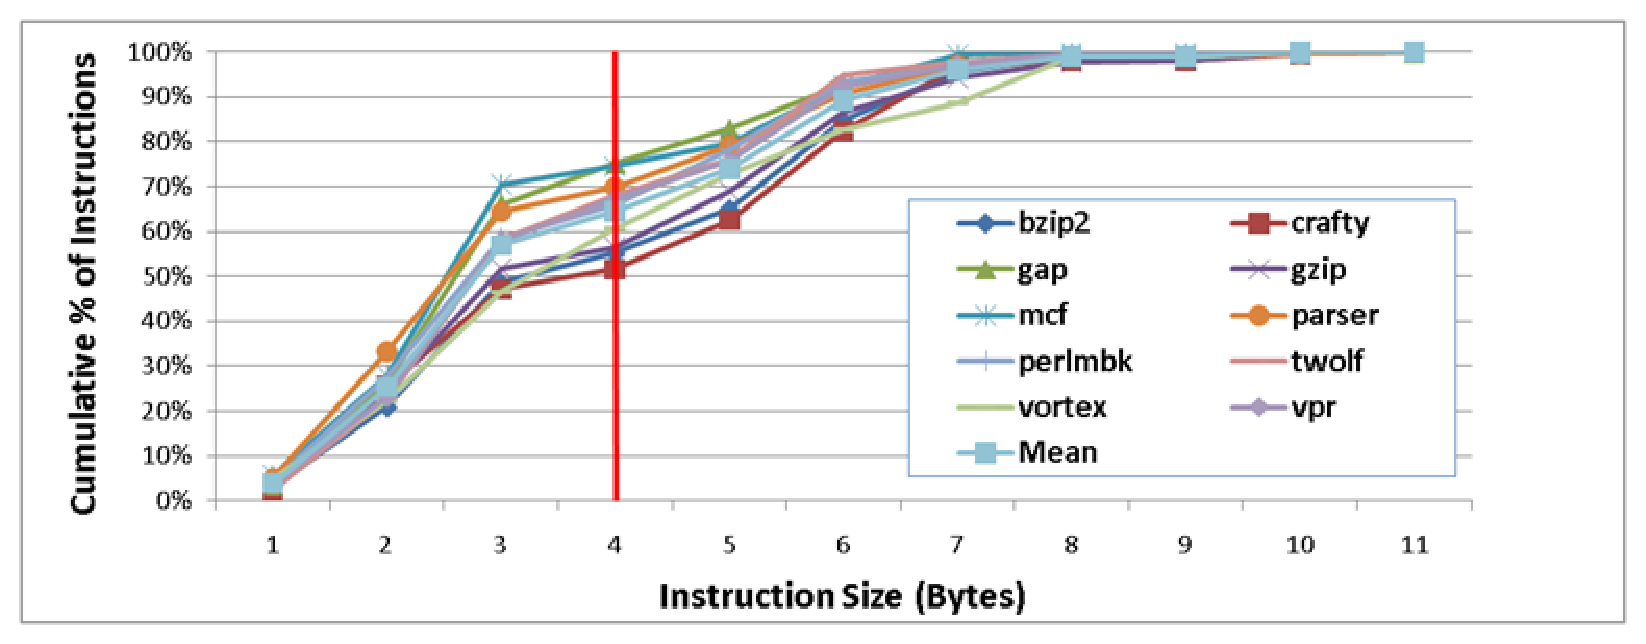
\includegraphics[scale=0.5]{instsize.eps}
\caption{Instruction sizes for several benchmarks presented in a cumulative basis.}
\end{figure}

This leaves two options for how to transfer control to the instrumentation code.
We must either use a technique entirely distinct from the idea of using a single
unconditional branch to execute the control transfer or we must somehow alter the application code so
that it can accommodate a single large control instruction that is larger than
the original amount of space available at the instrumentation point. One alternative
technique for transferring control flow could be to use a series of branches,
where the instruction in the instrumentation point is a small branch that
transfers control to a larger intermediate branch. This
method is unsatisfactory because the smallest traditional unconditional branch instruction available
on the x86 platform is 2 bytes in length, yet there are
instrumentation points with only a single byte available to them. \textbf{(COMMENT: Put the percetage of instruction under 2 bytes)}.
Besides, this technique would
require additional space to be available in close proximity to the instrumentation points since these
smaller branches are also very short reaching. 

Another option is the method proposed by the BIRD project \cite{nanda2006bird}, which
proposes the use of the single-byte \begin{it}INT3\end{it} instruction when a larger traditional
branch won't fit within the specified area. This instruction is functionally
perfect for static instrumentation because it consumes only a single byte and
allows us to transfer control to an arbitrary location by registering an
exception haThere will also be some overhead
associated with setting up a stack frame for the instrumentation function.ndler with the system. We performed a cursory study on this scheme
from an efficiency standpoint to determine whether it was worth further
investigation. On a small benchmark set, our implementation of using
\begin{it}INT3\end{it} only when 5-byte unconditional branches do not fit at
the instrumentation point introduces slowdown of at least 100X for
even a simple task of counting the number of executions of each basic block in the code. As one might
expect, this mechanism is unsuitable for efficient instrumentation since the
 heavyweight system call conventions are being invoked on a fairly regular basis.

In PIX, we use reorganization of the code at the function level so that
there is enough space at every instrumentation point to accommodate a 5-byte
jump. Specifically, the steps in whole function relocation includes \textit{function displacement}, \textit{linking function entry points},
\textit{branch conversion} and \textit{instruction padding}. Figure \ref{Figure:Relocation} presents the flow of information on 
this process with a simple example function in the original text section of an executable.

\begin{figure}[ht]
\centering
\caption[Optional caption for list of figures]
{The steps taken in order to prepare a function for instrumentation which collects
the memory addresses of an application.}
\subfigure[Original instruction sequence.]{
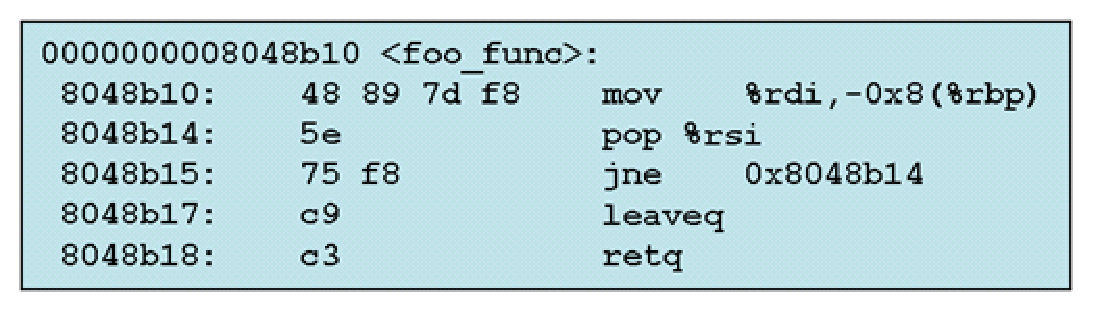
\includegraphics[scale=0.38]{funcp1.eps}
\label{Figure:funcp1}
}
\subfigure[Instructions after linking function entries.]{
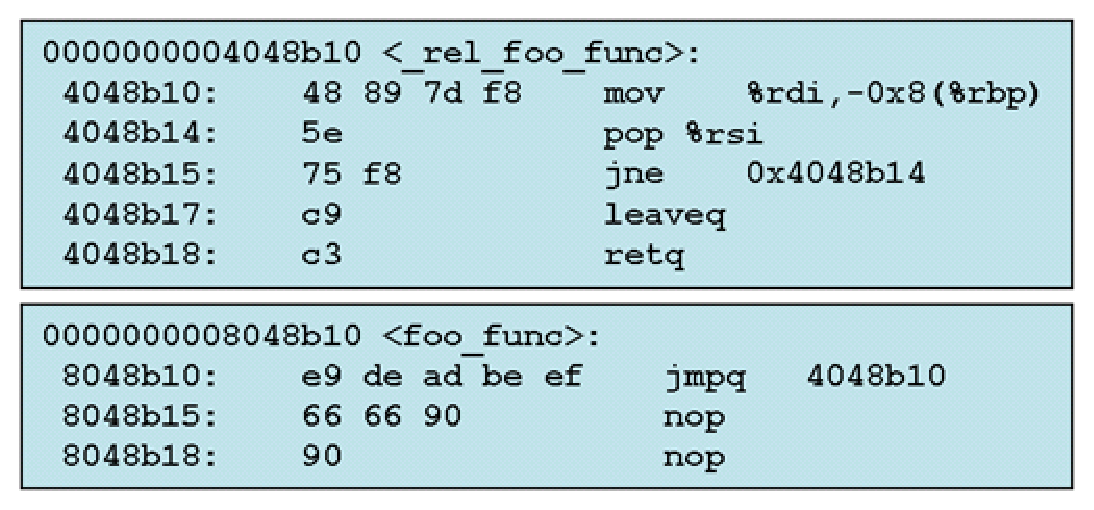
\includegraphics[scale=0.38]{funcp2.eps}
\label{Figure:funcp2}
}
\subfigure[Instructions after branch conversion.]{
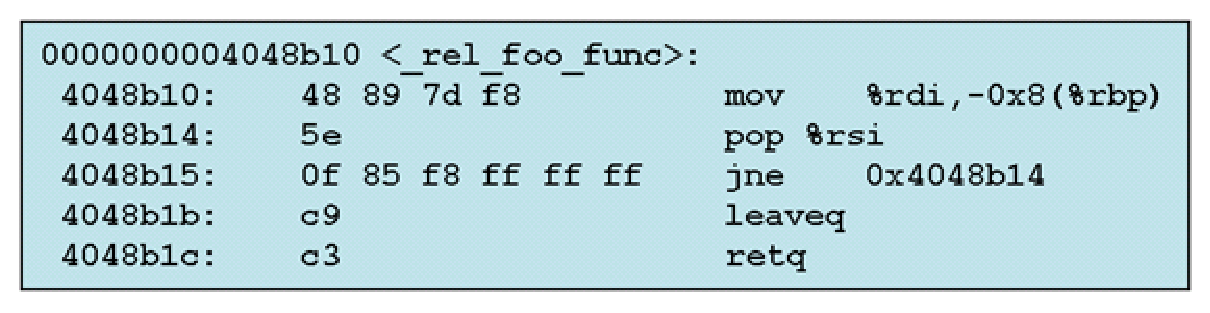
\includegraphics[scale=0.34]{funcp3.eps}
\label{Figure:funcp3}
}
\subfigure[Instructions after padding.]{
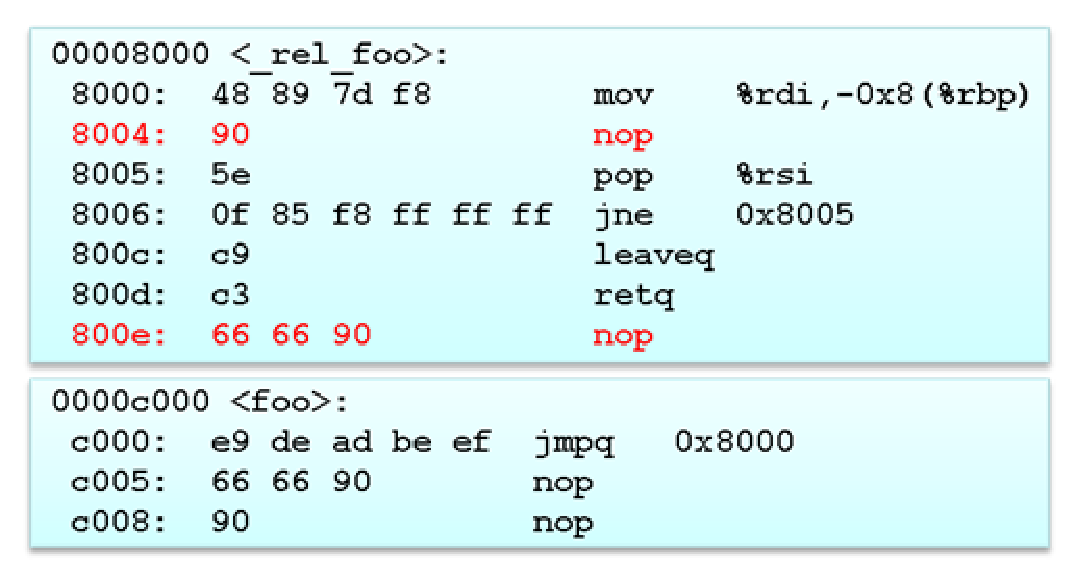
\includegraphics[scale=0.34]{funcp4.eps}
\label{Figure:funcp4}
}
\subfigure[Relocated function body.]{
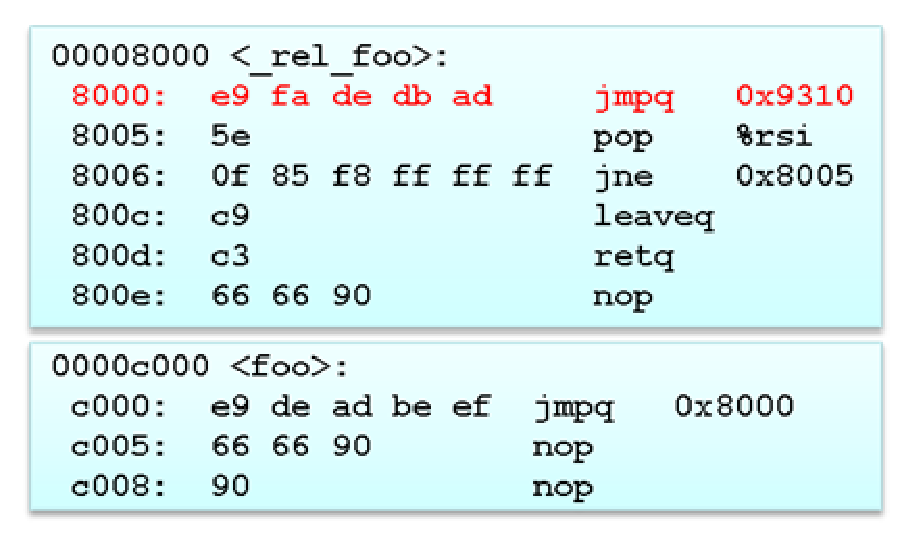
\includegraphics[scale=0.34]{funcp5.eps}
\label{Figure:funcp5}
}
\label{Figure:Relocation}
\end{figure}


\textit{Function Displacement} relocates the contents of the entire function to an area of the text section allocated
for the instrumentation. Since functions are often packed tightly together, it is generally not possible to
expand the size of a function without disturbing the entry points of another function using the original location of a function. 
\textit{Linking Function Entries} places an unconditional branch at the former function entry point that transfers control
to the new relocated function entry point. Most references to the entry point of a function are in the form of function calls, which
routinely are indirect references (i.e. their value is computed or looked up at runtime) and are difficult to resolve
prior to runtime. \textit{Branch Conversion} converts each short conditional branch in the relocated function to the equivalent
5-byte branch instruction. Since the code is being reorganized in the next step which may strain the limits of
smaller 8-bit or 16-bit offsets, we convert all branches to use 32-bit offsets so that the targets of each branch
will still be reachable without having the need to further reorganize the code. Note that there is opportunity
here to reduce space by using the smallest branch offset size that accommodates the branch, but we chose to use a single 
mechanism to simplify the implementation and optimize the space usage in the future. \textit{Instruction Padding} pads
the instruction at each instrumentation point with \begin{it}nop\end{it} instructions so that a 5-byte branch can fit
 according to the needs of the instrumentation. 

There are several ways that whole function relocation may adversely affect 
the performance of the instrumented executable independent of the overhead
that will be imposed by the additional instrumentation code. Each function call
now has an extra control interruption associated with it since control must be passed first to the original function entry
point and then to the relocated function entry point. In addition it is possible that using 32-bit offsets for every branch rather than
some smaller number of bits has an overhead associated with it. And since the code is being reorganized and expanded, 
we might destroy some positive alignment and size optimizations that the compiler might have made on the instructions in the
function.

To quantify the impact of whole function relocation and the other organizational changes we make
on the performance of applications, we show the results of experiments
where we generated executables in which functions are relocated and branches are converted to use 32-bit offsets, 
instruction padding is applied. This is basically the overhead of the transformations applied to the executable 
before any instrumentation code is inserted. We compared the performance of several applications to
the performance of the original executables. The overhead on the SPECINT 2000 benchmarks never exceeds 3.4\%, with an average
overhead of 0.8\%. Thus the basic overhead incurred by the code reorganization in PIX to accomodate all instrumentation points is
well within reason and does not represent a major hurdle for efficiency.

\subsection{Efficient Instrumentation Snippets}

In most instrumentation tools, the tasks accomplished by the instrumentation tool are accomplished by allowing the user
to transfer control from instrumentation points to the functions provided by the user, typically
via a shared library or some object code. Since these instrumentation functions are delivered via a shared library or other
object code, the instrumentation tool developer has the advantage to use a software devlepment toolchain and can
write the code in a language that compiles to the underlying object code. However, such delivery mechanism is heavyweight due to 
the overhead of a function invocation including saving the complete machine state for all possibles cases. In cases where
efficiency is important, it is more desirable to insert small sequences of assembly code to perform a task and only
save a small subset of machine state that will be affected rather than relying entirely on more heavyweight instrumentation functions.

Consider the example of an instrumentation point where we wish to increment a counter that resides in memory. 
In order to accompish this task with an instrumentation snippet, we transfer control to the
instrumentation point's trampoline which will save the flag registers, update the counter in memory, restore
the flags register, then transfer control back to the application. Using an instrumentation function, prior to performing
the task the trampoline must save the flag registers, any registers used by the function, and perform pushing an entry to the call stack.
This would also require at least 2 more jump instructions to enter and exit the instrumentation function. 
Furthermore these control flow transfers generally use the call/return paradigm, which in addition to changing the
application's program counter will also store and retreive information about the function call site onto the stack. 
The use of the instrumentation function is also more likely to pollute the instruction cache more than using a compact
instrumentation snippet. For an instrumentation snippet the application code must contend with the trampoline code
only, whereas using an instrumentation function puts the function code into contention with the other two as well. Hence, 
instrumentation functions tend to be more heaviweight solution, which would not be as appropriate when efficiency is considered
in instrumentation. Using simple snippets rather than instrumentation functions allows us to more efficiently gather 
asynchronous program information, which intuitively can be thought of as any information that could be dumped to
disk an processed offline. The Gao et. al. \cite{gao2005aliter} demostrates that using lightweight instrumentation snippets to buffer information
which is later processed by more heavyweight instrumentation functions in batches is an efficient yet entirely lossless way of processing asynchronous
program information. The avaialability of instrumentation snippets gives tool developers the flexibility to choose 
depending on their performance goals and software engineering needs.

% move this to overview section
The call stack during execution requires protection from the instrumentation code because compilers will often optimize a leaf function
by not explicitly creating a stack frame for the local function data to operate in. This optimization is safe for the application because during its
normal execution a leaf function will never call another function and thus its errant stack contents can never be smashed. In the case of an instrumentation
tool that calls an instrumentation function from a leaf, this guarantee no longer holds. Thus, the area above the stack needs to be protected when
an instrumentation function is called from a leaf function. During the disassembly of a function, PIX notes whether it is a leaf function (i.e. whether it contains any call
instructions). Later, during instrumentation, it automatically protects the stack contents for any instrumentation function calls that are made by
incrementing the stack pointer by a fixed safe amount, which has the effect of giving the leaf function a large stack frame while the instrumentation
function's stack frame uses the stack.
